\documentclass[tikz]{standalone}
\usepackage{tikz-cd}
\usetikzlibrary{matrix,arrows,arrows.meta,calc,backgrounds}
\usepackage{amsmath,amssymb}

\begin{document}
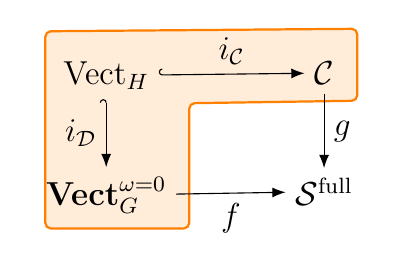
\begin{tikzpicture}[font=\large]
  \matrix (m) [matrix of math nodes, row sep=2.5em, column sep=4em] {
    \mathrm{Vect}_{H} & \mathcal{C} \\
    \mathbf{Vect}_{G}^{\omega=0} & \mathcal{S}^{\text{full}} \\
  };

  \path
    (m-1-1) edge[{Hooks[right]}-{Latex}] node[above] {$i_{\mathcal{C}}$} (m-1-2)
    (m-1-1) edge[{Hooks[left]}-{Latex}] node[left]  {$i_{\mathcal{D}}$} (m-2-1)
    (m-1-2) edge[-{Latex}]               node[right] {$g$} (m-2-2)
    (m-2-1) edge[-{Latex}]               node[below] {$f$} (m-2-2);

  \begin{scope}[on background layer]
    \fill[orange!15, rounded corners=2pt]
      ($(m-1-1)+(-22pt,  16pt)$) --
      ($(m-1-2)+( 12pt,  16pt)$) --
      ($(m-1-2)+( 12pt, -10pt)$) --
      ($(m-1-1)+( 30pt, -10pt)$) --
      ($(m-2-1)+( 30pt, -12pt)$) --
      ($(m-2-1)+(-22pt, -12pt)$) -- cycle;
    \draw[orange, thick, rounded corners=2pt]
      ($(m-1-1)+(-22pt,  16pt)$) --
      ($(m-1-2)+( 12pt,  16pt)$) --
      ($(m-1-2)+( 12pt, -10pt)$) --
      ($(m-1-1)+( 30pt, -10pt)$) --
      ($(m-2-1)+( 30pt, -12pt)$) --
      ($(m-2-1)+(-22pt, -12pt)$) -- cycle;
  \end{scope}
\end{tikzpicture}
\end{document}
